\chapter{Resultados e discussões}

\section{Aspecto da chama em regime permanente}

\subsection{Razão de equivalência 1}
O objetivo inicial foi avaliar o comportamento do reator de maneira qualitativa, variando-se a vazão volumétrica de ar para uma razão de equivalência constante. Os parâmetros de teste usados nos testes são mostrados na Tabela \ref{tab:phi1}.

\begin{table}[!htbp]
	\centering
	\small
	\renewcommand{\arraystretch}{1.3}
	\caption{Parâmetros do ensaio.}%
	\label{tab:phi1}
        \begin{tabular}{|l|c|c|c|c|}
        \hline
        \textbf{Posição do ventilador} & \multicolumn{1}{c|}{\textbf{7}} & \textbf{5}              & \textbf{3} & \textbf{1} \\ \hline
        ${Q}_{ar}$ (LPM)           & 229,8                           & 252,0                   & 272,3      & 286,6      \\ \hline
        $\Phi$                         & 1                               & 1                       & 1          & 1          \\ \hline
        $\dot{m}_{comb}$ ($g/s$)       & 0,748                           & 0,8205                  & 0,8865     & 0,9328     \\ \hline
        P (kW)                         & 13,76                           & 15,09                   & 16,31      & 17,16      \\ \hline
        TH (s)                         & 1                               & 1                       & 1          & 1          \\ \hline
        TL (s)                         & 127                             & 116                     & 107        & 102        \\ \hline
        $T_{admin, ar}$ (°C)           & 32                              & 31 & 31         & 31         \\ \hline
        \end{tabular}
    \vspace{2mm}
	\fonte{O autor.}
\end{table}

Para $\Phi = 1$, em 4 potências diferentes, o aspecto da chama é mostrado na Figura \ref{fig:4chamasphi1}. Em (a) a potência é a maior de todas, enquanto em (d) é a menor. Percebe-se que a altura da chama diminui conforme aumenta a potência. Esse fenômeno possivelmente decorre da geometria do queimador. Quanto maior a potência, mais ar é injetado no queimador, aumentando a vazão secundária de ar. Quando a vazão secundária aumenta, a chama é direcionada ao centro do reator, havendo inclusive a formação de vórtices, como mostrado na Figura \ref{fig:chamas}.

\begin{figure}[!ht]
    \centering
	\caption{Aspecto da chama para as 4 diferentes potências testadas.}
	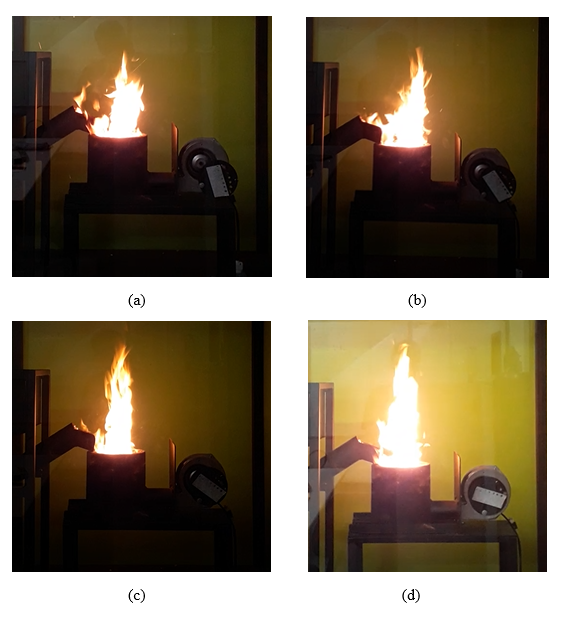
\includegraphics[scale=1]{Textuais/results/4chamas.png}
	\fonte{O autor (2022).}
	\label{fig:4chamasphi1}
\end{figure}

\begin{figure}[!ht]
	\centering
	\caption{Comparação entre a chama de menor potência (esquerda) e maior potência (direita).}
	\frame{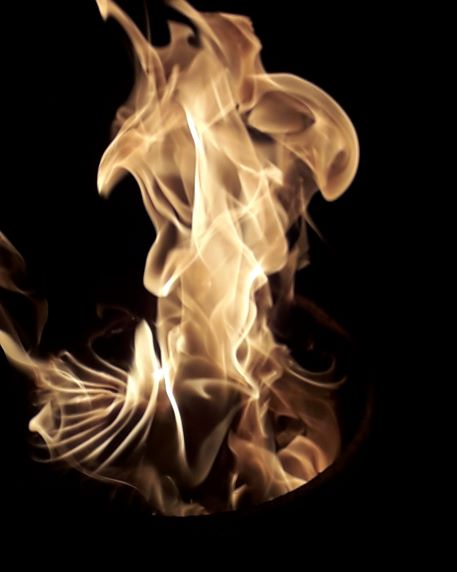
\includegraphics[scale=0.4]{Textuais/results/phi1pos7.jpg}}
	\frame{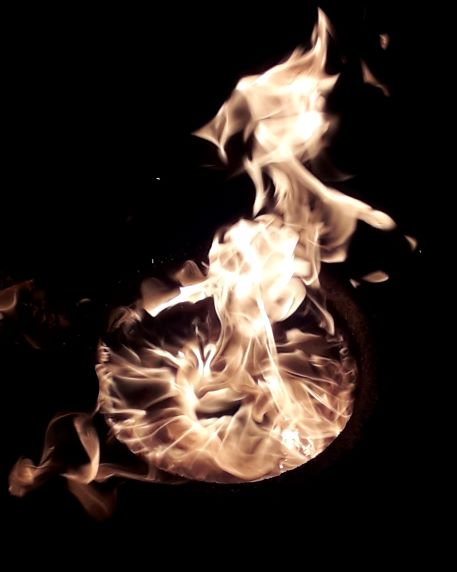
\includegraphics[scale=0.4]{Textuais/results/phi1pos1.jpg}}
	\fonte{O autor (2022).}
	\label{fig:chamas}
\end{figure}

Outro aspecto relevante na análise da chama é a distribuição dos pellets dentro do queimador. Na disposição em que o alimentador foi posicionado, o combustível tende a ficar acumulado do lado direito do queimador. Essa distribuição em alguns momentos tornou a chama assimétrica, principalmente para uma potência baixa, como verificado na Figura \ref{fig:assimetria} (potência 7).

\begin{figure}
	\centering
	\caption{Assimetria da chama.}
	\frame{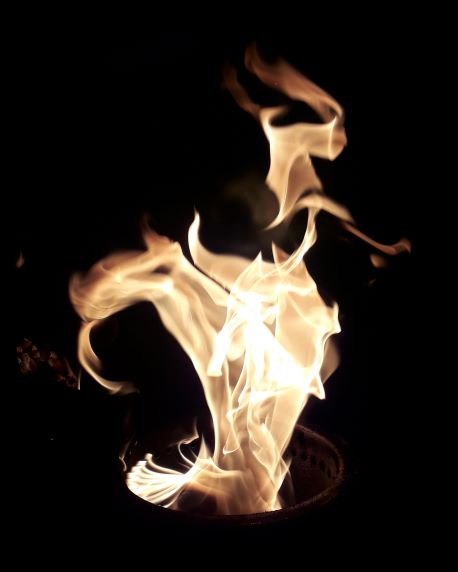
\includegraphics[scale=0.4]{Textuais/results/assimetria.jpg}}
	\fonte{O autor.}
	\label{fig:assimetria}
\end{figure}

\noindent Na Figura \ref{fig:assimetria} percebe-se que a injeção de ar secundária influencia mais a chama do lado da alimentação, em relação ao lado oposto. Isso se deve pois, tendo em vista que a vazão mássica é baixa, não há vazão suficiente de pellets para preencher a superfície da grade, fazendo com que o combustível se concentre no lado do alimentador.

Nesse ensaio, para cada potência considerou-se o tempo de estabilidade como sendo aproximadamente 40 minutos. Nesse intervalo, para todas as potências a chama se sustentou de maneira satisfatória. Entretanto, na potência mais alta foi constatado que o nível de pellets no queimador subiu ao longo do tempo. O equipamento foi mantido em regime automático por um tempo adicional de 20 minutos, a fim de verificar se o fenômeno persistiria. Ao final desse tempo, observou-se que o nível de pellets dentro do reator alcançava a injeção secundária de ar (Figura \ref{fig:transb}), o que certamente resultaria na extinção da chama. 

\begin{figure}[!ht]
	\centering
	\caption{Nível de pellets excessivo, alcançando o topo do reator.}
	\frame{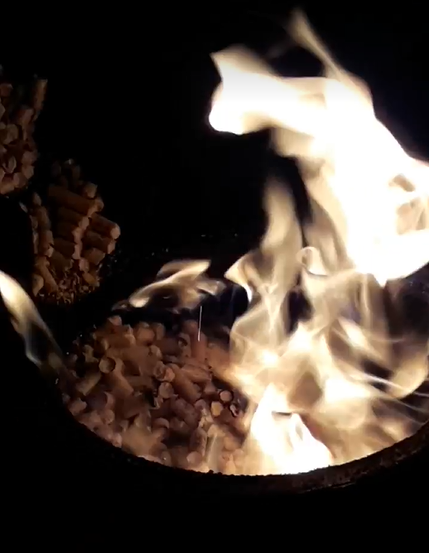
\includegraphics[scale=0.5]{Textuais/results/transbordando.png}}
	\fonte{O autor (2022).}
	\label{fig:transb}
\end{figure}

Esse transbordamento indica que a volatilização de uma certa quantidade de combustível não ocorre em tempo hábil antes de uma próxima carga ser inserida. Esse resultado aponta para a necessidade uma análise aprofundada da cinética química que rege as equações de volatilização e queima nesse reator, o que foge ao escopo do presente trabalho. Portanto, o ponto de potência 1 (maior potência) foi considerado como instável. 
\subsection{Razão de equivalência 0,7}
Para a razão de equivalência $\Phi = 0,7$ foram avaliadas três potências de operação, tendo em vista que no terceiro ensaio foi verificada uma leve tendência de o nível de pellets subir, sendo possível inferir que para a maior potência esse aumento de nível ocorreria de maneira semelhante ao que ocorreu para $\Phi=1$. Os parâmetros usados são mostrados na Tabela \ref{tab:phi0,7}.

\begin{table}[!ht]
	\centering
	\small
	\renewcommand{\arraystretch}{1.3}
	\caption{Parâmetros do ensaio.}%
	\label{tab:phi0,7}
        \begin{tabular}{|l|c|c|c|}
        \hline
        \textbf{Posição do ventilador} & \textbf{7} & \textbf{5} & \textbf{3} \\ \hline
        ${Q}_{ar}$ (LPM)           & 229,8      & 252,0      & 272,3      \\ \hline
        $\Phi$                         & 0,7        & 0,7        & 0,7        \\ \hline
        $\dot{m}_{comb}$ ($g/s$)       & 0,5236     & 0,5743     & 0,6206     \\ \hline
        P (kW)                         & 9,63       & 10,57      & 11,42      \\ \hline
        TH (s)                         & 1          & 1          & 0,5          \\ \hline
        TL (s)                         & 182        & 166           & 80          \\ \hline
        $T_{admin, ar}$ (°C)           & 29         & 28         & 29         \\ \hline
        \end{tabular}
    \vspace{2mm}
	\fonte{O autor (2022).}
\end{table}

O aspecto da chama para os três testes é mostrado na Figura \ref{fig:phi0,7tres}. Buscou-se capturar as imagens no momento em que a chama estabiliza, o que acontece aproximadamente na metade do tempo $TL$. Tal como na análise para $\Phi = 1$, de maneira geral a chama tende a ser mais alta para potências mais baixas, pelos mesmos motivos já comentados para aqueles resultados. 

\begin{figure}[!ht]
     \centering
        \caption{Aspecto da chama nos três diferentes testes.}
        \label{fig:phi0,7tres}
     \begin{subfigure}[b]{0.3\textwidth}
         \centering
         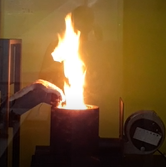
\includegraphics[width=\textwidth]{Textuais/results/0,7posicao7.png}
         \caption{Potência 7}
         \label{fig:pot7}
     \end{subfigure}
     \hfill
     \begin{subfigure}[b]{0.3\textwidth}
         \centering
         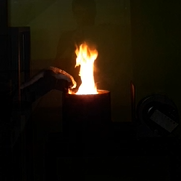
\includegraphics[width=\textwidth]{Textuais/results/0,7posicao5.png}
         \caption{Potência 5}
         \label{fig:pot5}
     \end{subfigure}
     \hfill
     \begin{subfigure}[b]{0.3\textwidth}
         \centering
         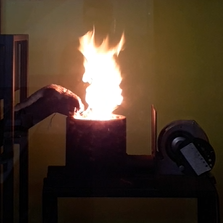
\includegraphics[width=\textwidth]{Textuais/results/0,7posicao3.png}
         \caption{Potência 3}
         \label{fig:pot3}
     \end{subfigure}
     \fonte{O autor (2022).}
\end{figure}

Uma particularidade dessa razão de equivalência é que o intervalo $TL$ se torna bastante longo, fazendo com que as propriedades da combustão variem consideravelmente nesse intervalo, o que se reflete no aspecto da chama. A sequência de imagens mostradas na Figura \ref{fig:perfilchama3_0,7} mostra a variação da chama ao longo do tempo, dentro de um intervalo $TL$, para a potência de 11,42 kW (posição 3 do ventilador). A primeira imagem foi capturada logo após a primeira alimentação, e as demais em intervalos periódicos de 15 segundos. Nessas condições, espera-se que as propriedades relativas à combustão (principalmente temperatura e emissões) variem mais a cada ciclo.  

\begin{figure}[!ht]
	\centering
	\caption{Perfil da chama em um mesmo intervalo $TL$.}
	\frame{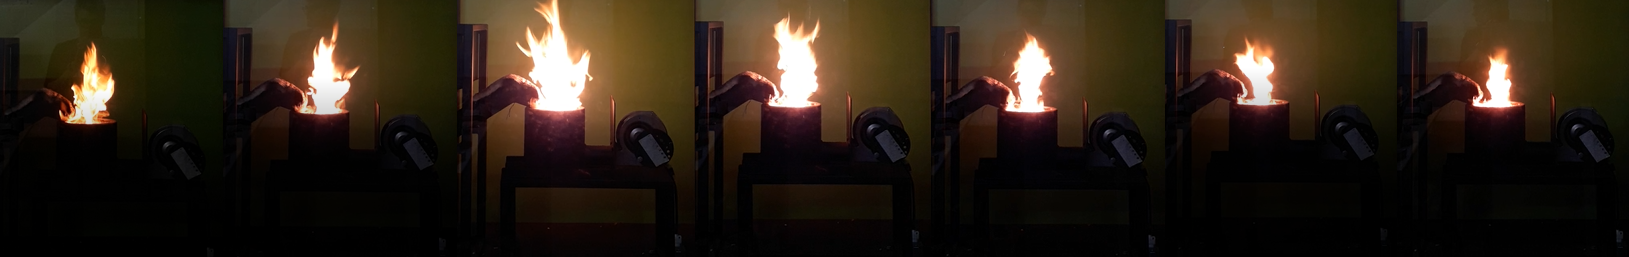
\includegraphics[scale=0.35]{Textuais/results/perfil_chama_0,7_3.png}}
	\fonte{O autor (2022).}
	\label{fig:perfilchama3_0,7}
\end{figure}

Em se tratando de combustão com mistura pobre ($\Phi < 1$), inicialmente esperava-se uma chama de coloração mais azulada. Todavia, como a massa de combustível no reator varia periodicamente, e a mistura acaba sendo bastante heterogênea, essa característica não foi observada. Somente ao final do experimento, quando o alimentador foi desligado e a massa de combustível contida no queimador espalhada uniformemente na grelha, foi possível observar essa chama de aspecto azulado (Figura \ref{fig:chamaazul}).

\begin{figure}[!ht]
	\centering
	\caption{Chama típica de misturas pobres, obtida no fim dos experimentos.}
	\frame{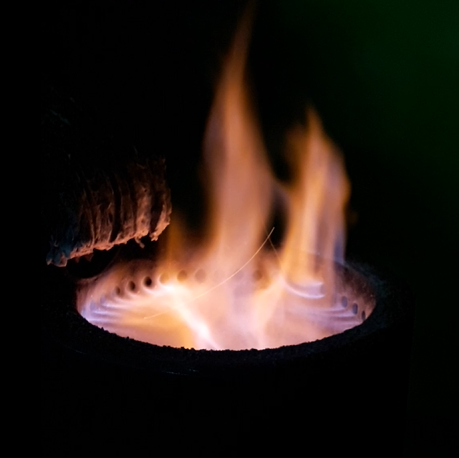
\includegraphics[scale=0.52]{Textuais/results/chama_azul.png}}
	\frame{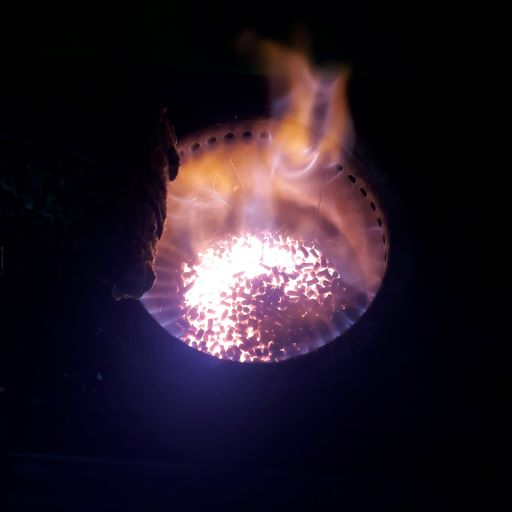
\includegraphics[scale=0.35]{Textuais/results/chama_azul_fundo.jpg}}
	\fonte{O autor (2022).}
	\label{fig:chamaazul}
\end{figure}

%%%%%%%%%%%%%%%%%%%%%%%%%%%%%%%%%%%%%%%%%%%%%%%%%%%%%%%%%%%%%%%%%%%%%%%%%%%%%%%%%%%%%%%%%%%%%%%%%%%%%%%%%%%%%%%%%%%%
\section{Temperatura e emissão de poluentes}

\subsection{Razão de equivalência 1}
Inicialmente buscou-se trabalhar com $\Phi = 1$, com a menor potência disponível (usando os parâmetros da segunda coluna da Tabela \ref{tab:phi1}). Entretanto, tendo em vista que a chaminé possui isolamento térmico, as temperaturas se elevaram, o que proporcionou a formação de uma chama muito alta (na Figura \ref{fig:demais} verifica-se que a chama termina no topo da chaminé). Essa chama, além de reduzir a vida útil do termopar, pode danificar a sonda de medição de gases. Para viabilizar as medições, optou-se então por trabalhar com $\Phi = 0,7$.

\begin{figure}[!ht]
	\centering
	\caption{Tentativa de medição para $\Phi = 1$, P = 13,76 kW.}
	\frame{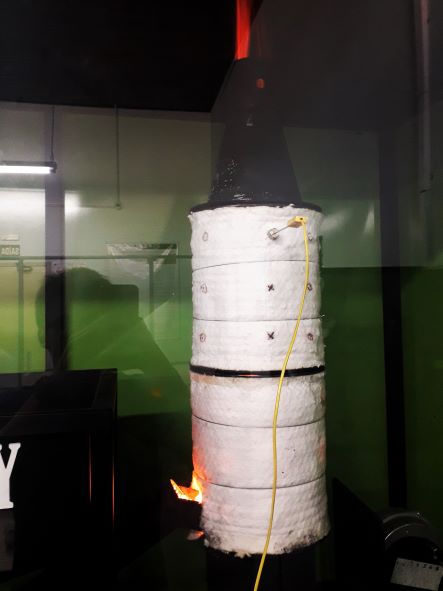
\includegraphics[scale=0.4]{Textuais/results/phi1poluentes.jpg}}
	\fonte{O autor (2022).}
	\label{fig:demais}
\end{figure}

\subsection{Razão de equivalência 0,7}
Os ensaios para $\Phi = 0,7$ foram realizados com base nos dados da Tabela \ref{tab:phi0,7}. Para cada caso, esperou-se a estabilização da temperatura dos gases dentro de um intervalo relativamente fixo. A  Figura \ref{fig:est_temp} mostra as temperaturas registradas dentro da faixa de estabilidade, sendo as linhas tracejadas a média para cada potência.

\begin{figure}[!ht]
	\centering
	\caption{Temperaturas registradas na estabilidade, para cada potência.}
	\frame{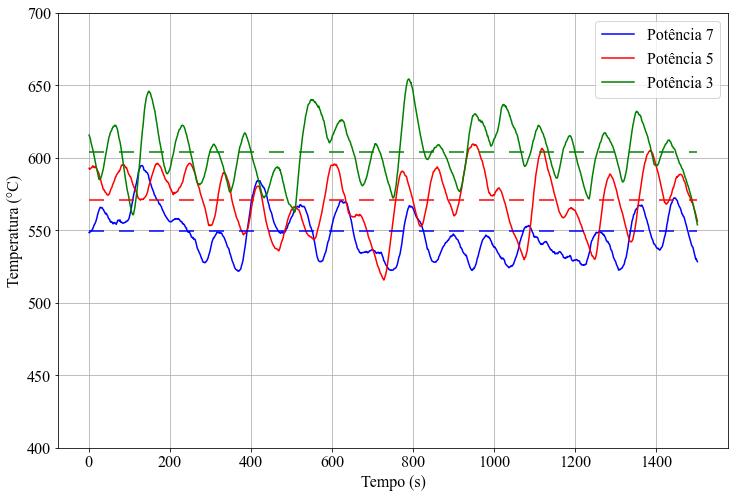
\includegraphics[scale=0.4]{Textuais/results/estabilizacao_temp.png}}
	\fonte{O autor (2022).}
	\label{fig:est_temp}
\end{figure}

Como esperado, observa-se que a temperatura média dos gases aumenta com a potência, sendo a diferença de temperatura entre as potências de 9,63 (potência 7) e 11,42 kW (potência 3) maior do que 60°C. A amplitude das oscilações varia principalmente devido à variação da massa de combustível despejada, que não é a mesma a cada ciclo tendo em vista que o tamanho dos pellets é variável. Outro aspecto que teve influência nesse parâmetro é a queima de pellets ainda na alimentação, antes de serem despejados no reator. Esse comportamento ocorre tendo em vista que a chama da injeção secundária se encontra muito próxima à alimentação, ocorrendo então uma queima parcial do combustível antes de ser introduzido no reator. Para corrigir esse aspecto, uma melhoria seria o projeto de uma portinhola, que permitisse que os pellets adentrassem o queimador, porém impedindo o contato da chama com o combustível cru.

A medição de emissões foi realizada para as três potências. Para cada uma foi possível determinar as curvas de \ch{CO2}, \ch{CO}, $\ch{NO}_{x}$, \ch{O2}, hidrocarbonetos e o perfil de temperatura registrado pelo termopar. Nos gráficos, as linhas verticais tracejadas em azul indicam o momento da alimentação de combustível. A primeira análise será feita para a potência 3 (Figura \ref{fig:emissoespot3}), tendo em vista ser a que mais nitidamente representa o comportamento dinâmico dos poluentes.

\begin{figure}[!ht]
	\centering
	\caption{Emissões para a potência 3 (11,42 kW).}
	\frame{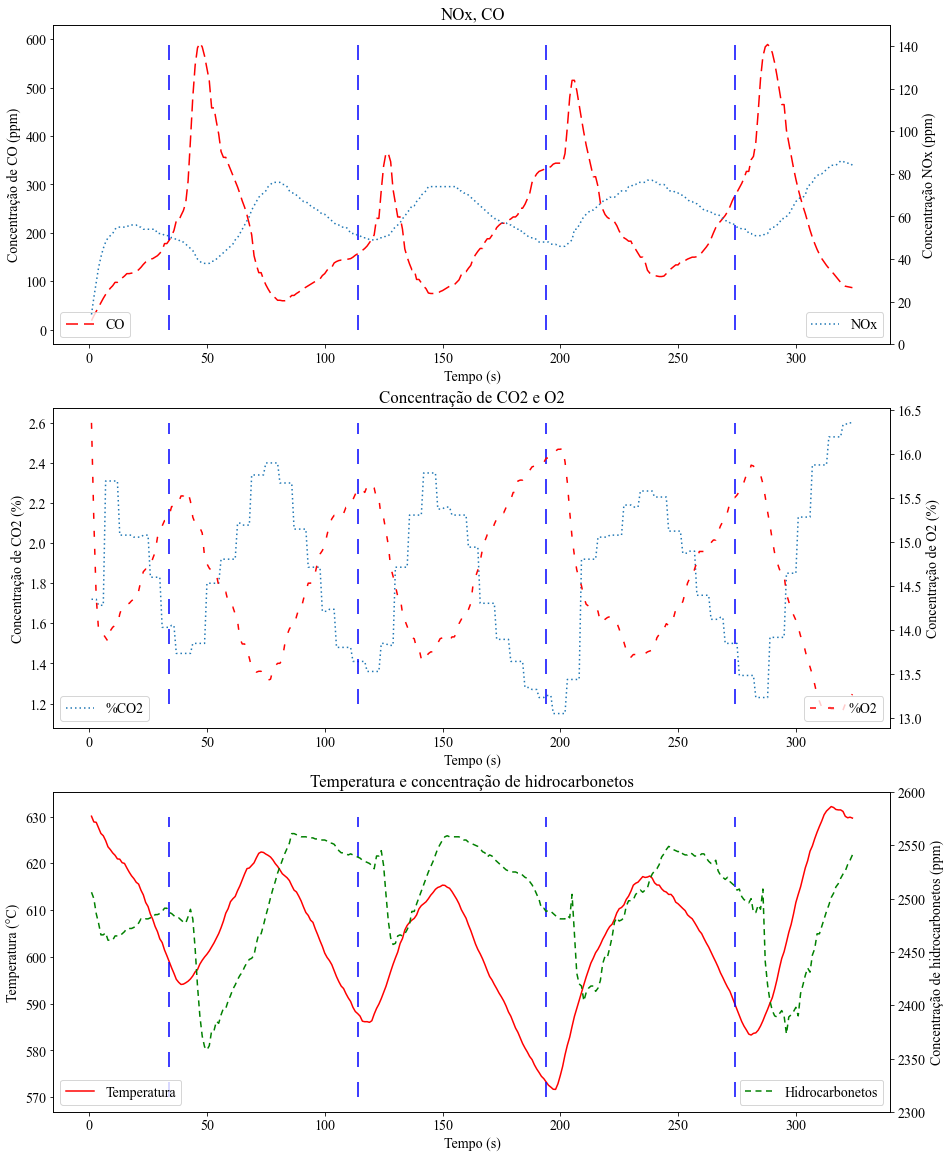
\includegraphics[scale=0.46]{Textuais/results/emissoespot3.png}}
	\fonte{O autor (2022).}
	\label{fig:emissoespot3}
\end{figure}

Do terceiro gráfico da Figura \ref{fig:emissoespot3} percebe-se que, logo após a alimentação de pellets, a temperatura tende a continuar caindo por um pequeno intervalo de tempo. Isso acontece pois a biomassa entra no reator relativamente fria e com alguma umidade, sendo necessário um certo tempo para o conjunto ganhar calor. Assim que o combustível inicia o desprendimento dos voláteis, a reação de combustão no topo do reator começa a se intensificar, o que aumenta a temperatura dos gases de combustão. Essa temperatura atinge um máximo aproximadamente na metade do intervalo $TL$. quando então começa a diminuir devido à diminuição de combustível, com consequente diminuição da volatilização e da combustão. A temperatura cai até aproximadamente o valor inicial, quando então ocorre uma nova alimentação, e o ciclo se repete.

Partindo para análise da concentração de \ch{CO} (primeiro gráfico), percebe-se que sua concentração aumenta abruptamente após o despejo da biomassa, devido justamente ao caráter transiente das reações no reator. À medida em que o tempo passa e a temperatura aumenta, a reação de formação de dióxido de carbono (concentração mostrada no segundo gráfico) é favorecida, tendo em vista que ambas as concentrações de \ch{CO} e \ch{O2} são altas. Dessa forma, a concentração de \ch{CO2} aumenta enquanto as de \ch{CO} e \ch{O2} diminuem. Verifica-se um máximo na concentração de \ch{CO2} que é bastante próximo ao ponto de máxima temperatura. Conforme o tempo passa e a quantidade de combustível disponível é menor, os níveis de \ch{CO2} diminuem, enquanto os níveis de \ch{CO} gradativamente voltam a aumentar. Um dos fatores responsáveis pela oxidação do \ch{CO} após a injeção de combustível pode ser a presença do vapor de água proveniente da secagem do combustível na reação. Turns (2013) ressalta que "[...] a oxidação de \ch{CO} é um processo relativamente lento, a menos que espécies químicas contendo hidrogênio estejam presentes. Até mesmo pequenas quantidades de \ch{H2O} ou \ch{H2} podem ter um grande efeito na taxa de oxidação". 

A concentração de $\ch{NO}_x$ registrada no primeiro gráfico varia proporcionalmente à temperatura. Tendo em vista que a formação de $\ch{NO}_x$ é favorecida com o aumento de temperatura \cite{Turns}, o resultado obtido é condizente com a literatura. 

Para as demais potências os gráficos são mostrados nas Figuras \ref{fig:emissoespot5} e \ref{fig:emissoespot7}.

\begin{figure}[!ht]
	\centering
	\caption{Emissões para a potência 5 (10,57 kW).}
	\frame{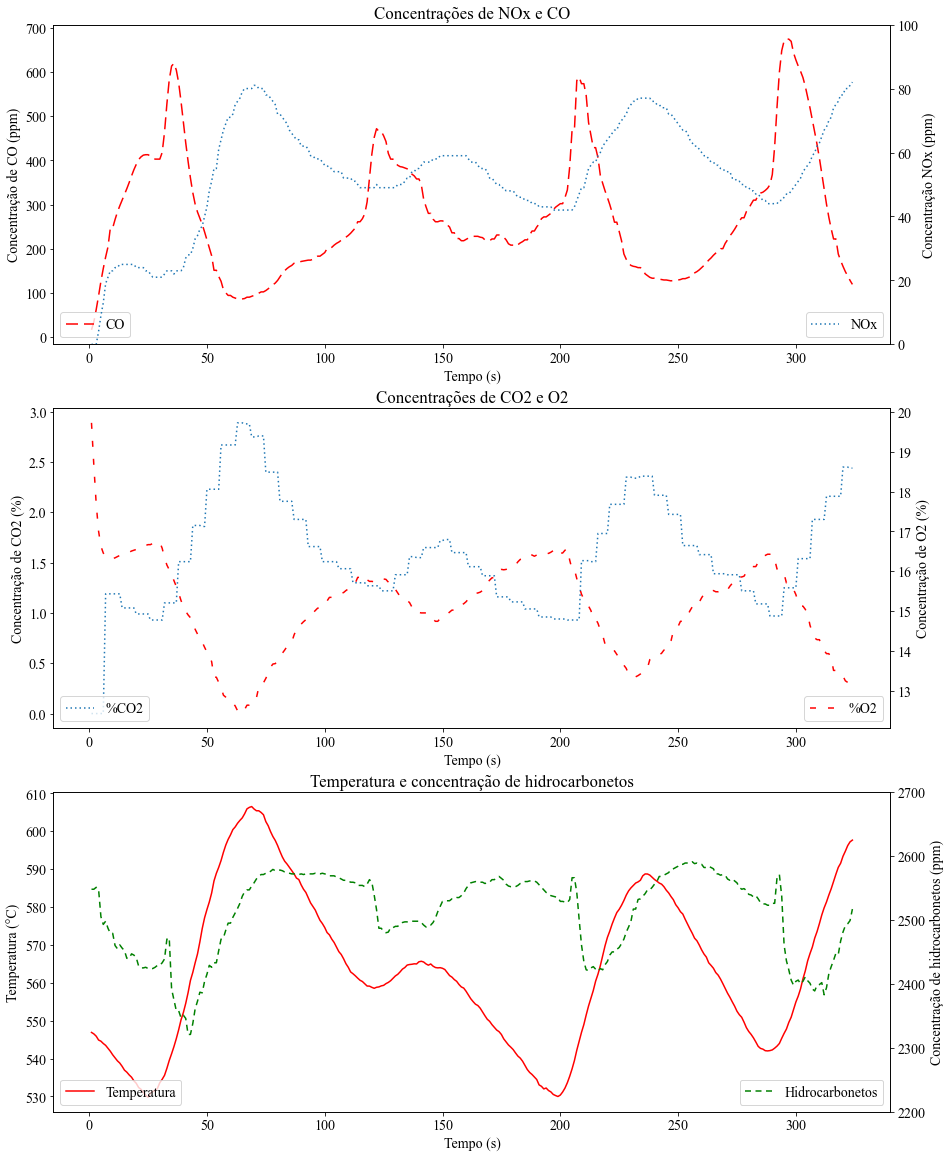
\includegraphics[scale=0.46]{Textuais/results/emissoespot5.png}}
	\fonte{O autor (2022).}
	\label{fig:emissoespot5}
\end{figure}

\begin{figure}[!ht]
	\centering
	\caption{Emissões para a potência 7 (9,63 kW).}
	\frame{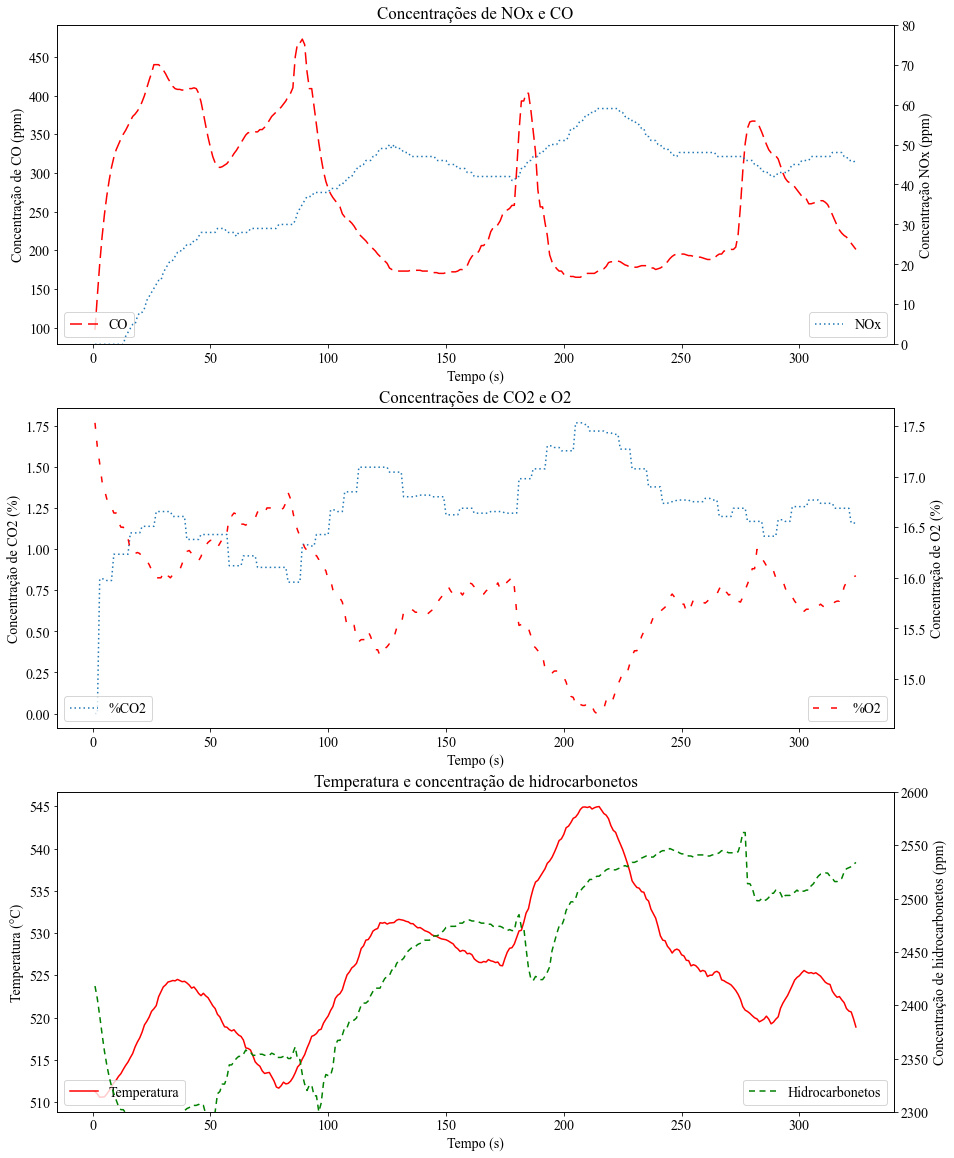
\includegraphics[scale=0.46]{Textuais/results/emissoespot7.png}}
	\fonte{O autor (2022).}
	\label{fig:emissoespot7}
\end{figure}

Nesses gráficos percebe-se que o comportamento é bastante semelhante ao já descrito para a potência de 11,42 kW. Fica evidente nos três gráficos a forte dependência da formação de $\ch{NO}_x$ com a temperatura, e também a simetria entre as curvas de \ch{CO2} e \ch{O2}. Para nenhum dos gráficos foi obtida uma conclusão precisa acerca da concentração de hidrocarbonetos, cuja oxidação é fortemente relacionada à presença de radicais O e H. 

Em termos da média nos períodos medidos, os resultados obtidos são mostrados na Tabela \ref{tab:emissoesmedias}.

\begin{table}[!htbp]
	\centering
	\small
	\renewcommand{\arraystretch}{1.3}
	\caption{Valores médios de emissões.}%
	\label{tab:emissoesmedias}
        \begin{tabular}{|l|c|c|c|}
        \hline
        \textbf{Posição do ventilador} & \textbf{7} & \textbf{5} & \textbf{3} \\ \hline
        \ch{CO} (ppm)                       & 265        & 275        & 215        \\ \hline
        $\ch{NO}_x$ (ppm)                      & 40         & 53         & 60         \\ \hline
        \ch{CO2} (\%)                    & 1,25       & 1,58       & 1,85       \\ \hline
        $C_xH_y$ (ppm)                 & 2438       & 2509       & 2494       \\ \hline
        \ch{O2} (\%)                     & 15,84      & 15,12      & 14,58      \\ \hline
        $T_{med}$ (°C)                 & 525,79     & 563,54     & 604,5      \\ \hline
        \end{tabular}
    \vspace{2mm}
	\fonte{O autor (2022).}
\end{table}

No Brasil, o CONAMA (Conselho Nacional do Meio Ambiente) regula os níveis máximos de emissão de poluentes atmosféricos para fontes fixas. A atual resolução (CONAMA 382/06) é válida para licenças de instalação requeridas após 02/01/2007, portanto será usada como base na presente análise. Para processos de geração de calor a partir da combustão externa de derivados de madeira, os limites são mostrados na Figura \ref{fig:CONAMA}.

\begin{figure}[!ht]
     \centering
        \caption{Limites para emissões de poluentes, de acordo com a Resolução CONAMA 382/06.}
        \label{fig:CONAMA}
     \begin{subfigure}[b]{0.8\linewidth}
         \centering
         \frame{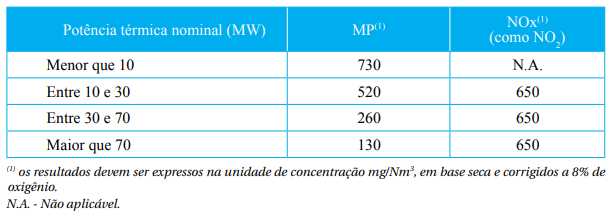
\includegraphics[width=\columnwidth]{Textuais/results/CONAMA_2.png}}
         \caption{}
         \label{fig:conama2}
     \end{subfigure}
     \hfill
     \begin{subfigure}{0.8\linewidth}
         \centering
         \frame{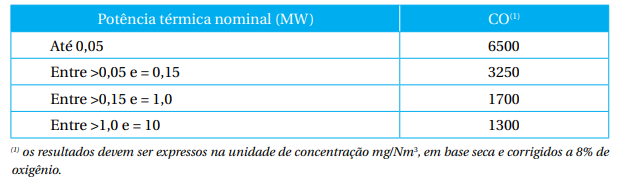
\includegraphics[width=\columnwidth]{Textuais/results/CONAMA_1.png}}
         \caption{}
         \label{fig:conama1}
     \end{subfigure}
     \fonte{CONAMA (2006).}
\end{figure}

\noindent A norma exige um fator de correção, dado pela Equação \eqref{eq:correcao}.
\begin{equation} \label{eq:correcao}
    C_R = \frac{21-O_R}{21-O_M} C_M
\end{equation}

\noindent Na Equação:
\begin{enumerate}
    \item $C_R$: concentração do poluente corrigida pela condição da resolução;
    \item $O_R$: porcentagem de oxigênio de referência (nesse caso 8\%);
    \item $O_M$: porcentagem de oxigênio medida durante a amostragem;
    \item $C_M$: concentração do poluente medida.
\end{enumerate}

A Tabela \ref{tab:comparacaoCONAMA} relaciona os dados de \ch{CO} obtidos no presente estudo (corrigidos a partir da Equação \eqref{eq:correcao}) com os limites requeridos pela norma. Os dados de $\ch{NO}_x$ não foram avaliados tendo em vista que a potência da aplicação é menor do que 10 MW. A conversão de ppm para $mg/Nm^3$ é realizada usando a Equação \eqref{eq:ppm}, adotando-se $MW_{CO} = 28,01$ kg/kmol.
\begin{equation} \label{eq:ppm}
    CO \left[\frac{mg}{Nm^3}\right] = CO [ppm]\cdot \frac{MW_{CO}}{22,4}
\end{equation}

\begin{table}[!htbp]
	\centering
	\small
	\renewcommand{\arraystretch}{1.3}
	\caption{Conversão dos valores obtidos no presente estudo para comparação com a Resolução.}%
	\label{tab:comparacaoCONAMA}
        \begin{tabular}{|l|c|c|c|c|}
        \hline
        \textbf{Posição do ventilador} & CO (ppm) & CO ($mg/Nm^3$) & $O_2$ (\%) & $C_{CO, R} (mg/Nm^3)$ \\ \hline
        \textbf{7}                     & 265      & 331,37            & 15,84        & 834,84                \\ \hline
        \textbf{5}                     & 275       & 343,87             & 15,12         & 760,26                \\ \hline
        \textbf{3}                     & 215     & 268,85           & 14,58       & 544,39                \\ \hline
        \end{tabular}
    \vspace{2mm}
	\fonte{O autor.}
\end{table}

Percebe-se que os valores obtidos para $C_{CO,R}$ encontram-se significativamente abaixo do limite previsto na Resolução (de 6500 $mg/Nm^3$), indicando que o equipamento atende a norma vigente de limite de emissões no Brasil. 


